% theory/00-modelo.tex — T05: model, definitions and running example
% Project SemComV1 · feature 001-codigo-trayectoria · 2026-10-13
% Notation follows specs/001-codigo-trayectoria/plan.md §2 (constitution P7).
% Every number in Section 4 is produced by theory/ejemplo_semana.py (constitution P4.1).
\documentclass[11pt]{article}
\usepackage[margin=1in]{geometry}
\usepackage{amsmath,amssymb,amsthm,mathtools}
\usepackage{booktabs}
\usepackage{tikz}
\usetikzlibrary{arrows.meta,positioning}
\usepackage[hidelinks]{hyperref}
\newcommand{\doi}[1]{doi:\,\url{#1}}

\newtheorem{definition}{Definition}
\newtheorem{lemma}{Lemma}
\newtheorem{theorem}{Theorem}
\newtheorem{assumption}{Assumption}
\theoremstyle{remark}
\newtheorem{remark}{Remark}
\newtheorem{example}{Example}

\newcommand{\M}{\mathcal{M}}
\newcommand{\Pset}{\Pi}
\newcommand{\E}{\mathbb{E}}
\newcommand{\D}{D}
\DeclareMathOperator*{\argmax}{arg\,max}

\title{Path Codes on Shared Knowledge Graphs\\[2pt]\large Part 0: Model, Definitions and Running Example}
\author{R.~Sandoval Ar\'echiga (working notes)}
\date{October 13, 2026 --- v0.1}

\begin{document}
\maketitle

\begin{abstract}
These notes fix the model and notation used by all subsequent results. A transmitter and a receiver share a labelled directed graph; a meaning is conveyed by a walk on it. The walk-to-meaning map is a synonymous mapping in the sense of Niu and Zhang~\cite{niu2025}, but here it is \emph{induced by the graph structure}. We define path codes with and without decoder memory, the misalignment between transmitter and receiver graphs, and the geodesic semantic distortion. A ten-node example is worked out in full.
\end{abstract}

\section{Standing assumptions}

\begin{assumption}[Finite rooted DAG]\label{as:dag}
The graph is finite, directed and acyclic, with a unique root $r$ and a non-empty set of terminal nodes (nodes with out-degree $0$). Every node is reachable from $r$.
\end{assumption}

\begin{assumption}[Node-Markov routing]\label{as:markov}
At every non-terminal node $v$ the next edge is drawn from a distribution $p(\cdot\mid v)$ that depends on $v$ only.
\end{assumption}

\begin{assumption}[Meaning at completion]\label{as:meaning}
A meaning is attached to complete walks (from $r$ to a terminal), not to prefixes.
\end{assumption}

Assumption~\ref{as:dag} guarantees that the set of complete walks is finite, so all quantities below are finite sums. Knowledge graphs usually contain cycles; if walks are bounded in length by $L$, unrolling the graph into $L$ layers yields a DAG that satisfies Assumption~\ref{as:dag}, and all results apply to it. Assumption~\ref{as:meaning} is relaxed in the hierarchical setting of Part~3, where prefixes carry coarse meanings.

\section{Definitions}

\begin{definition}[Trajectory network]\label{def:tn}
A trajectory network is a tuple $G=(V,E,r,T,\ell,p)$ where $(V,E)$ satisfies Assumption~\ref{as:dag}, $T\subset V$ is the set of terminals, $\ell:V\to\Sigma$ is a labelling with values in a finite alphabet $\Sigma$, and $p$ is a routing kernel: for every $v\in V\setminus T$, $p(\cdot\mid v)$ is a probability distribution on the out-neighbours of $v$.
\end{definition}

\begin{definition}[Walks and path measure]\label{def:path}
A \emph{complete walk} is a sequence $\pi=(v_0,v_1,\dots,v_k)$ with $v_0=r$, $(v_{t-1},v_t)\in E$ and $v_k\in T$. Let $\Pset_G$ denote the set of complete walks. The routing kernel induces the \emph{path measure}
\begin{equation}\label{eq:pathmeasure}
P(\pi)=\prod_{t=1}^{k} p(v_t\mid v_{t-1}),\qquad \pi\in\Pset_G .
\end{equation}
A random complete walk with law $P$ is denoted $\Pi$.
\end{definition}

\begin{definition}[Meaning map, preimage, synonymy]\label{def:meaning}
A \emph{meaning map} is a surjection $\mu:\Pset_G\to\M$ onto a finite set of meanings. The \emph{preimage} of $m\in\M$ is $\Pset(m)=\mu^{-1}(m)$. The random meaning is $M=\mu(\Pi)$, with law
\begin{equation}\label{eq:meaninglaw}
P_M(m)=\sum_{\pi\in\Pset(m)}P(\pi).
\end{equation}
Two walks are \emph{synonymous} if they have the same image under $\mu$. The network exhibits synonymy if $|\Pset(m)|\ge 2$ for some $m$.
\end{definition}

\begin{remark}[Relation to synonymous mappings]\label{rem:niu}
The preimages $\{\Pset(m)\}_{m\in\M}$ partition $\Pset_G$, so $\mu$ is a synonymous mapping in the sense of~\cite[Def.~2.1]{niu2025}, with walks playing the role of syntactic symbols. In particular, $H(M)$ is their semantic entropy $H_s$, and coding each meaning directly achieves it~\cite[Thm.~6.8]{niu2025},~\cite{liang2025}. Two features have no counterpart in the unstructured setting: (i) a walk is produced and consumed \emph{decision by decision}, so a decoder may or may not keep memory of the prefix; (ii) transmitter and receiver may hold \emph{different} networks.
\end{remark}

Because $\mu$ is a function of $\Pi$, the chain rule gives the decomposition used throughout:
\begin{equation}\label{eq:chain}
H(\Pi)=H(M)+H(\Pi\mid M).
\end{equation}

\begin{definition}[Path codes]\label{def:codes}
A \emph{path code} for $(G,\mu)$ is a pair $(f,\mathcal{C})$ where $f:\M\to\Pset_G$ is a selection with $f(m)\in\Pset(m)$, and $\mathcal{C}$ is a sequential binary code that describes $f(m)$ one decision at a time, so that the receiver reconstructs the walk while traversing it. The code is
\begin{itemize}
\item \emph{native} if the coding distribution used for the decision at $v_{t-1}$ is the shared kernel $p(\cdot\mid v_{t-1})$;
\item \emph{adapted} if it uses a kernel agreed for the code, which may differ from $p$; an adapted code is \emph{memoryless} if that kernel depends on the current node only, and \emph{with memory} if it may depend on the prefix $(v_0,\dots,v_{t-1})$.
\end{itemize}
The rate of a path code is its expected length $L=\E[\,|\mathcal{C}(f(M))|\,]$.
\end{definition}

\begin{lemma}[Cost of a walk; arithmetic coding~\cite{rissanen1979,witten1987,cover2006}]\label{lem:cost}
For any distribution $Q$ on $\Pset_G$ that factorises as a product of sequential conditionals, there is a prefix-free sequential code with $|\mathcal{C}(\pi)|<-\log_2 Q(\pi)+2$ for every $\pi$ with $Q(\pi)>0$. In particular, a native path code spends $-\log_2 p(v_t\mid v_{t-1})$ bits per decision, up to $2$ bits overall, and a node with out-degree $1$ costs $0$ bits.
\end{lemma}

\begin{definition}[Transmitter and receiver networks; misalignment]\label{def:misalign}
The transmitter holds $G_S$ with routing $p_S$ and the receiver holds $G_R$ with routing $q_R$, over a common node set $V$ and a common meaning map $\mu$. Let $P_S$ and $Q_R$ be the induced path measures. The \emph{misalignment} is
\begin{equation}\label{eq:A}
A=\D(P_S\,\|\,Q_R)=\sum_{\pi}P_S(\pi)\log_2\frac{P_S(\pi)}{Q_R(\pi)}\in[0,\infty].
\end{equation}
An edge missing in $G_R$ is encoded as $q_R(e\mid v)=0$. The \emph{edited nodes} are $V_\Delta=\{v: p_S(\cdot\mid v)\neq q_R(\cdot\mid v)\}$.
\end{definition}

\begin{definition}[Visit measure]\label{def:visits}
$\nu_S(v)=\Pr_{P_S}[\,v\in\Pi\,]$ is the probability that a walk drawn from $P_S$ visits $v$. In a DAG each node is visited at most once, so $\nu_S(v)$ also equals the expected number of visits.
\end{definition}

\begin{definition}[Geodesic semantic distortion]\label{def:dist}
Let $O$ be a connected undirected graph on $\M$ (an ontology or concept graph). The \emph{geodesic distortion} is $d_O(m,\hat m)$, the length of a shortest path between $m$ and $\hat m$ in $O$. It is \emph{ultrametric} if $d_O(m,m'')\le\max\{d_O(m,m'),d_O(m',m'')\}$ for all triples, as happens on the leaves of a rooted tree of height $h$ with $d(m,m')=h-\operatorname{depth}(\operatorname{lca}(m,m'))$.
\end{definition}

\begin{definition}[Quotients]\label{def:quotient}
A partition $\mathcal{Q}=\{B_1,\dots,B_J\}$ of $\M$ is a \emph{quotient codebook}. Its diameter is $\operatorname{diam}(\mathcal{Q})=\max_j\max_{m,m'\in B_j}d_O(m,m')$. Given representatives $b_j\in B_j$, the decoder outputs $b_j$ whenever $M\in B_j$. The quotient rate is $H(\mathcal{Q})=-\sum_j P_M(B_j)\log_2P_M(B_j)$.
\end{definition}

\section{Statements proved in Parts 1--4 (for orientation only)}

\begin{itemize}
\item \textbf{Part 1 (price of memory).} Native path codes have rate $H(M)+\E[g(M)]$, where $g(m)=\log_2\bigl(P_M(m)/\max_{\pi\in\Pset(m)}P(\pi)\bigr)$ and $0\le\E[g(M)]\le H(\Pset\mid M)$. Adapted codes attain $H(M)$; they need no decoder memory when the meaning is endpoint-determined, and may need it when the meaning depends on the route. Bits-back~\cite{frey1997} attains $H(M)$ in an amortised sense.
\item \textbf{Part 2 (structural misalignment).} $A=\sum_v\nu_S(v)\,\D\bigl(p_S(\cdot\mid v)\,\|\,q_R(\cdot\mid v)\bigr)$, with two-sided local bounds; $A$ splits into a meaning-level term, the semantic relative entropy of~\cite[Def.~4.1]{niu2025}, and a phrasing-level term. Routing, topological and label edits respectively cost bits, are detected, and cause silent errors.
\item \textbf{Part 3 (geodesic rate--distortion).} Quotient codes achieve points of the rate--distortion region, are tight at both ends and strictly suboptimal in between. Successive refinability under ultrametric distortion holds numerically for uniform sources (conjecture) and fails for non-uniform ones.
\item \textbf{Part 4 (Weaver's levels).} Technical, semantic and effectiveness levels form a chain of quotients with rates $H(\Pi)\ge H(M)\ge H(a(M))$.
\end{itemize}

\section{Running example: ``what day is today''}\label{sec:example}

\paragraph{Network.} Ten nodes (Fig.~\ref{fig:week}). From the root $r$ a single edge leads to $c$, ``according to the calendar''. At $c$ the speaker chooses a frame: $a$ = ``today is'' with probability $0.6$, or $b$ = ``tomorrow is'' with probability $0.4$. From $a$ the walk ends at Monday, Tuesday or Wednesday with probabilities $(0.5,0.3,0.2)$. From $b$ it ends at Tuesday$'$, Wednesday$'$ or Thursday with the same probabilities. The meaning $\mu$ is \emph{the day it is today}, so ``today is Monday'' and ``tomorrow is Tuesday'' are synonymous. The synonymy is induced by the graph: it comes from the structure of the two frames, not from a list.

\begin{figure}[h]
\centering
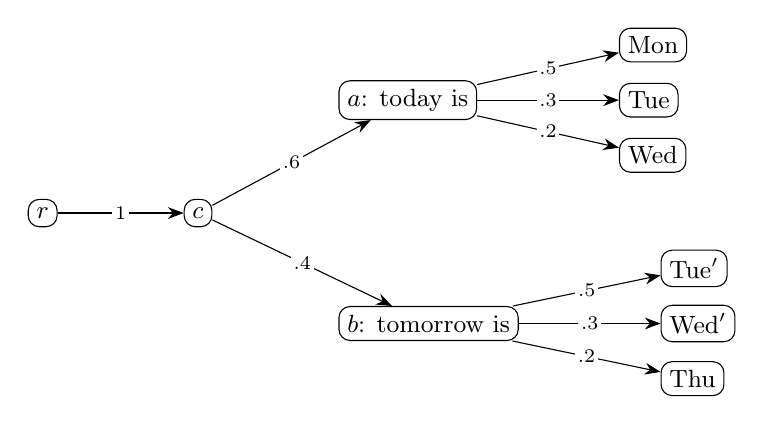
\begin{tikzpicture}[>={Stealth[length=2mm]},node distance=8mm and 16mm,
  every node/.style={draw,rounded corners,inner sep=3pt,font=\small}]
  \node (r) {$r$};
  \node (c) [right=of r] {$c$};
  \node (a) [above right=10mm and 16mm of c] {$a$: today is};
  \node (b) [below right=10mm and 16mm of c] {$b$: tomorrow is};
  \node (L) [right=18mm of a,yshift=7mm] {Mon};
  \node (Ma) [right=18mm of a] {Tue};
  \node (Wa) [right=18mm of a,yshift=-7mm] {Wed};
  \node (Mb) [right=18mm of b,yshift=7mm] {Tue$'$};
  \node (Wb) [right=18mm of b] {Wed$'$};
  \node (J) [right=18mm of b,yshift=-7mm] {Thu};
  \begin{scope}[every node/.style={font=\scriptsize,fill=white,inner sep=1pt}]
  \draw[->] (r)--node{1} (c);
  \draw[->] (c)--node{.6} (a); \draw[->] (c)--node{.4} (b);
  \draw[->] (a)--node{.5} (L); \draw[->] (a)--node{.3} (Ma); \draw[->] (a)--node{.2} (Wa);
  \draw[->] (b)--node{.5} (Mb); \draw[->] (b)--node{.3} (Wb); \draw[->] (b)--node{.2} (J);
  \end{scope}
\end{tikzpicture}
\caption{Running example. Meaning = the day it is today; ``today is Mon'' and ``tomorrow is Tue$'$'' are synonymous.}
\label{fig:week}
\end{figure}

\noindent\begin{minipage}{\linewidth}
\paragraph{Path and meaning laws.}
\begin{center}
\begin{tabular}{lccc}
\toprule
Walk $\pi$ & $P(\pi)$ & $\mu(\pi)$ & $-\log_2 P(\pi)$ \\
\midrule
$r\,c\,a\,$Mon & $0.30$ & Monday & $1.737$\\
$r\,c\,a\,$Tue & $0.18$ & Tuesday & $2.474$\\
$r\,c\,a\,$Wed & $0.12$ & Wednesday & $3.059$\\
$r\,c\,b\,$Tue$'$ & $0.20$ & Monday & $2.322$\\
$r\,c\,b\,$Wed$'$ & $0.12$ & Tuesday & $3.059$\\
$r\,c\,b\,$Thu & $0.08$ & Wednesday & $3.644$\\
\bottomrule
\end{tabular}
\end{center}
\end{minipage}

Hence $P_M=(0.5,0.3,0.2)$ for (Monday, Tuesday, Wednesday), $H(\Pi)=2.456$, $H(M)=1.485$ and $H(\Pi\mid M)=0.971$ bits, in agreement with~\eqref{eq:chain}.

\paragraph{Cost of a walk (Lemma~\ref{lem:cost}).} The walk $r\,c\,a\,$Mon costs $0+0.737+1=1.737$ bits. The first decision is free because $r$ has out-degree~$1$.

\paragraph{Price of memory.} For every meaning, the most probable walk goes through $a$, and
\[
\frac{P_M(m)}{\max_{\pi\in\Pset(m)}P(\pi)}=\frac{1}{0.6}\quad\text{for all } m.
\]
Thus $g(m)=\log_2(1/0.6)=0.737$ bits for all $m$, and the best native code has rate $L_0=2.222=H(M)+0.737$ bits. The excess is exactly the cost of the decision at $c$ between ``today is'' and ``tomorrow is'', which carries no meaning. An adapted code knows that the selected walks always pass through $a$, codes that decision with probability $1$, and attains $H(M)=1.485$; here it needs no memory (Part~1). Here $\E[g(M)]=0.737<H(\Pi\mid M)=0.971$: the upper bound of Part~1 is not tight because the conditional law of walks given the meaning is $(0.6,0.4)$, not uniform.

\paragraph{Misalignment (Part 2).}
\begin{itemize}
\item \emph{Probability edit.} Suppose the receiver routes uniformly at $a$, $q_R(\cdot\mid a)=(1/3,1/3,1/3)$, and agrees elsewhere. Then $V_\Delta=\{a\}$, $\nu_S(a)=0.6$, and
\[
A=0.6\cdot\D\bigl((0.5,0.3,0.2)\,\|\,(\tfrac13,\tfrac13,\tfrac13)\bigr)=0.060\ \text{bits},
\]
below the bound $0.6\log_2 3=0.951$. It splits as $0.036$ bits at the level of meanings plus $0.024$ bits that only path codes pay.
\item \emph{Missing edge.} If the receiver lacks the edge $b\to$ Thu, the walk $r\,c\,b\,$Thu has $Q_R=0$ and $A=\infty$ under the full path measure: the receiver detects an impossible walk with no checksum. An adapted code that always selects walks through $a$ never uses that edge. The structural mismatch is invisible to it.
\end{itemize}

\paragraph{Geodesic distortion (Part 3).} Let $O$ be the path Monday--Tuesday--Wednesday, so $d_O(\text{Mon},\text{Tue})=d_O(\text{Tue},\text{Wed})=1$ and $d_O(\text{Mon},\text{Wed})=2$. The quotient $\{\{\text{Mon},\text{Tue}\},\{\text{Wed}\}\}$ has diameter $1$ and rate $H(0.8,0.2)=0.722$ bits. With the best representative (Monday) its expected distortion is $0.3$. The alternative
$\{\{\text{Mon}\},$ $\{\text{Tue},\text{Wed}\}\}$ also has diameter $1$, with rate $1.000$ bit and distortion $0.2$. Part~3 compares both with the Blahut--Arimoto value of $R(D)$~\cite{blahut1972}: at $D=0.3$, $R(D)=0.439$ bits.

\begin{thebibliography}{9}
\bibitem{niu2025} K.~Niu and P.~Zhang, \emph{The Mathematical Theory of Semantic Communication}. SpringerBriefs in Computer Science, 2025. \doi{10.1007/978-981-96-5132-0}.
\bibitem{liang2025} Z.~Liang, K.~Niu, J.~Xu, and P.~Zhang, ``Semantic arithmetic coding using synonymous mappings,'' \emph{Entropy}, vol.~27, no.~4, art.~429, 2025. \doi{10.3390/e27040429}.
\bibitem{rissanen1979} J.~Rissanen and G.~G.~Langdon, ``Arithmetic coding,'' \emph{IBM J. Res. Dev.}, 1979. \doi{10.1147/rd.232.0149}.
\bibitem{witten1987} I.~H.~Witten, R.~M.~Neal, and J.~G.~Cleary, ``Arithmetic coding for data compression,'' \emph{Commun. ACM}, vol.~30, no.~6, pp.~520--540, 1987. \doi{10.1145/214762.214771}.
\bibitem{cover2006} T.~M.~Cover and J.~A.~Thomas, \emph{Elements of Information Theory}. Wiley, 2005. \doi{10.1002/047174882X}.
\bibitem{frey1997} B.~J.~Frey, ``Efficient stochastic source coding and an application to a Bayesian network source model,'' \emph{Comput. J.}, vol.~40, no.~2--3, pp.~157--165, 1997. \doi{10.1093/comjnl/40.2_and_3.157}.
\bibitem{blahut1972} R.~E.~Blahut, ``Computation of channel capacity and rate-distortion functions,'' \emph{IEEE Trans. Inf. Theory}, vol.~18, no.~4, pp.~460--473, 1972. \doi{10.1109/TIT.1972.1054855}.
\end{thebibliography}

\end{document}
